\section{Background}
This section motivates \sys in relation to prior work.
Using the pilot study as inspiration, consider the following running example to describe the system and notation:

\begin{example}[Lead Prediction]\sloppy\label{ex:lead}
 Past clients are stored in a relational database:
\[
R(id, name, num\_emp, industry, region, successful)
\]
where $name$ is the company name, $num\_emp$ is the number of employees in the company, $industry$ is a categorical attribute that describes the industry segment, $region$ is a code indicating the region of the country the business is headquartered, and $is\_successful$ is a Boolean describing whether the company purchased the product.
\end{example}

\subsection{Machine Learning and Dirty Data}
The relationship between machine learning and dirty data is subtle, and we are not concerned about statistical noise or variance in the dataset.
Rather, we are interested in cases where an invariant that is expected to be true, i.e., a logical assertion about properties of the dataset, is violated leading unforseen biases in the way the records are featurized.
Featurization is the process that turns a relational record into a numerical vector.
For example, suppose we expect every $num\_emp \ne~NULL$, but the particular dataset we receive has null values.
Either the featurization program will error, or worse, it may not error and interpret $NULL$ as $0$.
However, semantically $NULL$ and $0$ refer to two very different concepts: a missing value, or a company with no employees.
Conversely, one can also construct cases where two values that have the same semantic meaning are mapped to different numerical representations.
Suppose the attribute $region$ has two representations for the western United States: $USWEST$ and $USW$. 
This would lead to two different feature values for records from the same region.

Fundamentally, performance of a model degrades when these violated invariants create a mismatch between the training and prediction environments~(Figure \ref{fig:error}):

\vspace{0.5em}\noindent\textbf{Training Errors: } Invariants that are expected to be true during prediction time are violated in the training dataset. In the running example, consider the case when $R$ is integrated from multiple previously collected datasets, where some of the datasets failed to record $num\_emp$. Assuming that there is no convenient way to retroactively determine the ground truth, the analyst has a couple options to handle this error: (1) drop all records with a missing  $num\_emp$ value, or (2) impute $num\_emp$ with a sensible default value.

\vspace{0.25em}\noindent\textbf{Prediction Errors: } Invariants that are expected to be true during training time are violated when the model is asked to predict a label for a new example. 
Consider the case where all of training examples recorded $num\_emp$, but a new test example has a null value.
Unlike in the training set, it may not be an acceptable solution to drop a prediction (i.e., the system fails to respond to a query).
So, the analyst has a couple different options to handle this error: (1) impute $num\_emp$ with a sensible default value and then predict, (2) apply a ``fail-safe'' prediction.

\begin{figure}[t]
% \vspace{-5pt}
\centering
 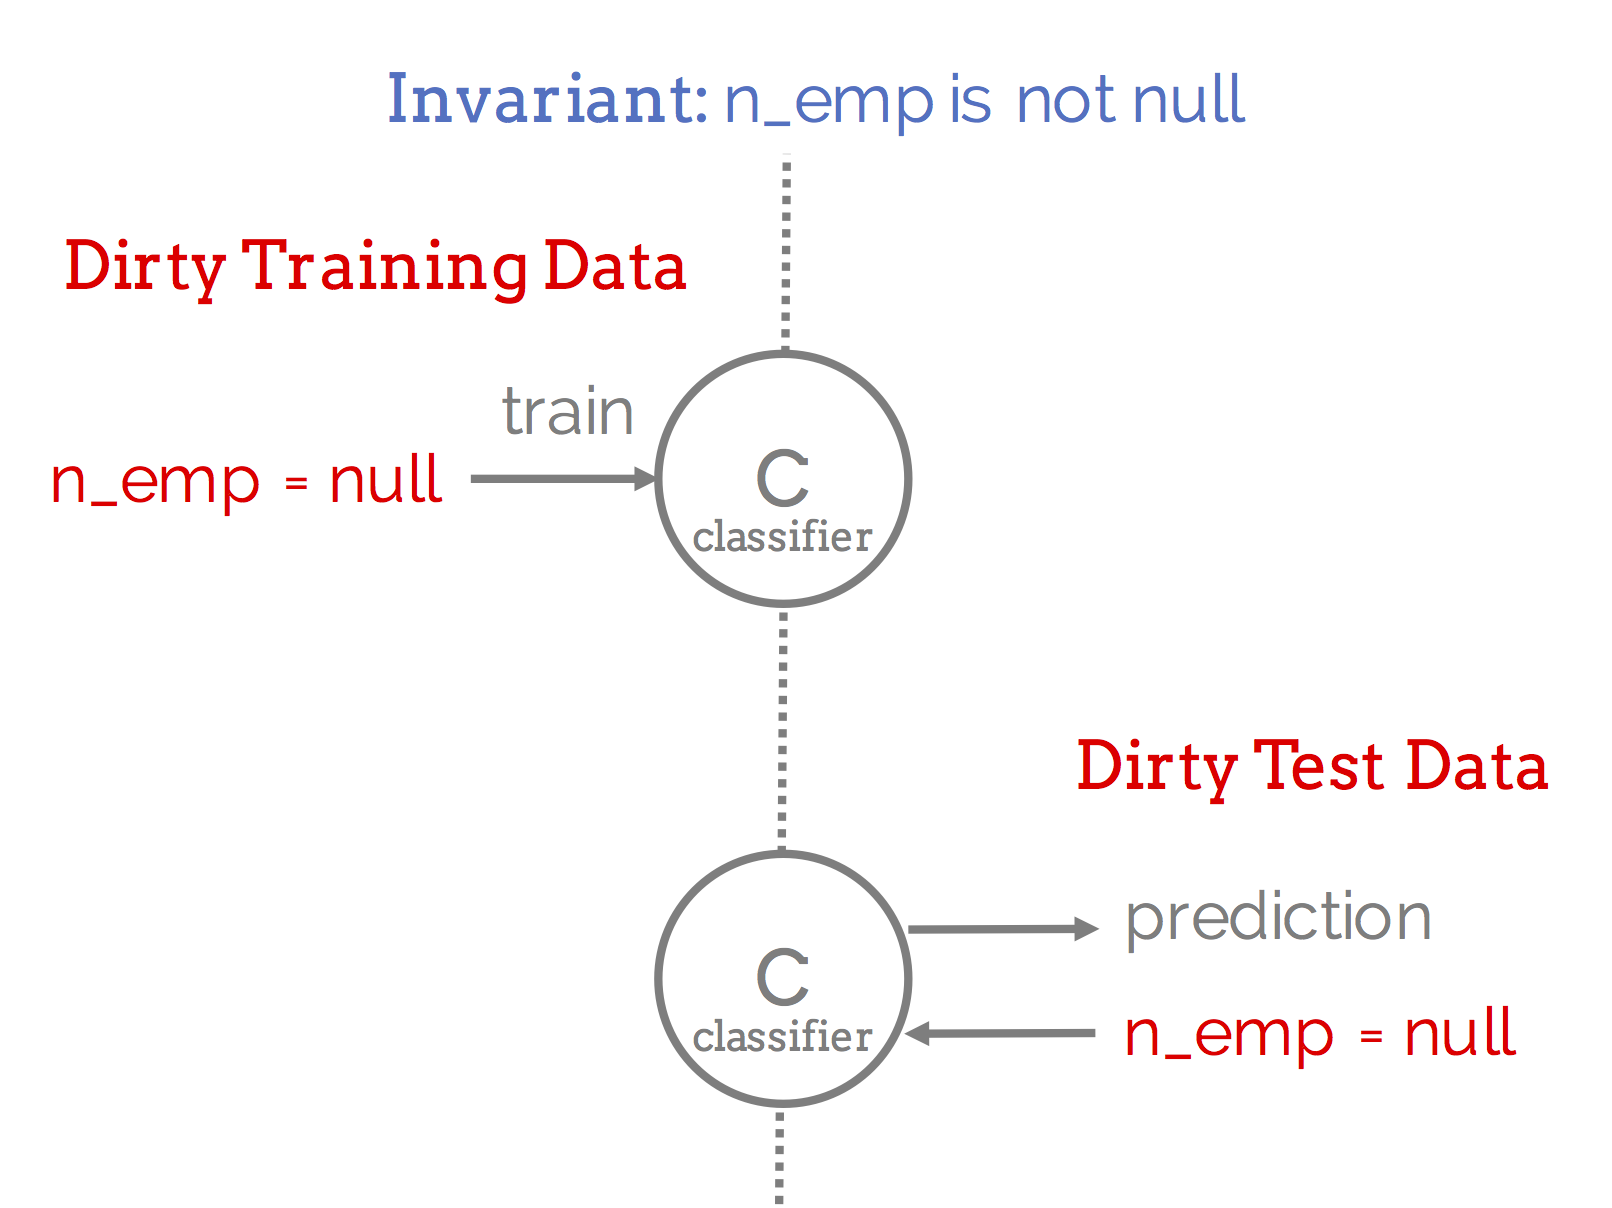
\includegraphics[width=0.8\columnwidth]{figures/training_and_pred_errors.png}
 \caption{Training errors are invariants that are expected to be true during prediction time are violated in the training dataset. Prediction errors are invariants that are expected to be true during training time are violated when the model is asked to predict a label for a new example. \sys is a tool to detect such violations and learns to perform a corrective action.
 \label{fig:error}}
\end{figure}

\vspace{0.5em}

This story becomes increasingly complicated as eventually we may want to integrate the new examples into the model and re-train--turning prediction errors into future training errors.
Already, for a missing value in $num\_emp$, there are four different choices the analyst can handle a violation (2 training $\times$ 2 prediction).
These four choices have to be evaluated for each possible error type based on its severity, data type, and predictive importance.
Recent surveys of data scientists suggest that the current procedure for making these choices is manual and ad-hoc~\cite{kandel2012, krishnan2016hilda}.
As ML applications are increasingly in the critical path, management systems that are resilient to errors by automatically making such choices are important.

In general, this is a challenging problem so to limit the scope, we focus on a particular instance classification problems where there exists an objective (uncorrupted by dirty data) measure of prediction accuracy, i.e., how well a particular label is predicted.
In many scenarios, such metrics are available.
Labels often represent directly observed user-behavior (e.g., sale vs. no sale, whether the user clicked a link etc.), and thus, are relatively consistent over the lifetime of an application.
We will use the signal from the labels to determine the right data cleaning choices to make.
The goal is to achieve this with minimal supervision from the data scientist.

\subsection{Possible Approaches}
\sys brings together generic, dataset-independent error detection with automatically learned repair strategies for ML applications.
We review how baseline techniques proposed in previous literature that could apply.


\vspace{0.5em}

\noindent\textbf{Automatic Repair: } 
The traditional relational approach to this problem to ignore the downstream model and clean the relation completely.
In the running example, suppose some of the values for $num\_emp$ are NULL and we want to train a classifier to predict $is\_successful$.
We would define a domain integrity constraint $num\_emp \ne~NULL$, and then propose a set of repairs to satisfy this constraint.
With no other information, this rule-based approach could in principle impute any non-null value from the domain to create a consistent relation.
To avoid this problem, we can adopt an approach like~\cite{prokoshyna2015combining} and select the imputations that minimize the statistical distance of the updated relation to an ideal distribution for the attribute, for example, an ideal power-law distribution.
This would impute values in such a way that $num\_emp$ matched a Zipfian distribution.

On its own this optimization approach has been empirically very successful, however, when we train a classifier on this data, counter-intuitive effects can occur.  
The data cleaning operation may break important correlations in the data and may introduce biases into the training data not present in test conditions. 
Consider the degenerate case where $num\_emp = NULL$ is perfectly correlated with one of the prediction classes--in this case, it may be better to NOT clean the data!
Similarly, consider the case where there is a very strong class imbalance.
When observing a record with $num\_emp = NULL$, rather than making a noisy prediction, it might be better to default to the most popular class. 
While more sophisticated statistical imputation techniques exist~\cite{schafer1998multiple}, they all have the same fundamental problem that the value imputation is divorced from the downstream classifier's predictive accuracy.

\vspace{0.5em}\noindent\textbf{Automatic Detection: } Rule-based techniques are dependent on the analyst defining the invariants, which might be challenging if the analyst cannot anticipate how future data might look.
There is a well-established line of literature on statistical anomaly detection~\cite{hellerstein2008quantitative}, and for the most part, these techniques are generic and dataset independent (up-to hyperparameters). Typically, such approaches identify \emph{outlier} records outside of some normal range of variance. However, the problem is that not all dirty data look like outliers. In the running example, there could truly be companies where $num\_emp = 0$. It has been shown that statistical anomaly detection techniques miss obvious errors in heterogeneous datasets with mixes of numerical, categorical, and string-valued data~\cite{DBLP:journals/pvldb/AbedjanCDFIOPST16}.

Therefore, we need a mix of statistical rules and logic rules to determine errors.
We explore to what extent we can derive these rules from data for routine errors. 
We surveyed 8 ML datasets used in Kaggle competitions and benchmarks in the UCI ML repository, and found that a majority of the non-statistical errors could be detected as \emph{domain integrity constraints}, i.e., disallowed values in single columns.
We apply a combination of heuristic checks for missing values and data type errors, and a neural network based error detector that identifies attribute values not likely to co-occur in the same record.

\vspace{0.5em}\noindent\textbf{Boosting: } There does not exist one single error detector or repair action that dominates, so which ones should an analyst choose? 
\sys models this problem as a boosting problem.
Rather than thinking of each of detector and repair pair as a data transformation, it thinks of each as generating a new ``classifier'' that provides some additional information.
The problem of selecting the top data pairs is equivalent to ensembling a subset of the classifiers as best as possible.
We choose a boosting framework to represent this problem due to the relatively minimal assumptions about the structure and implementation details of the user-specified classifier.
To construct the underlying library of cleaning operations we surveyed datasets on Kaggle and the UCI repository and built a library of data cleaning operations that supported common data cleaning tasks across the datasets.


